\documentclass[twoside,10pt]{article}
\usepackage{amsmath,amsfonts,amsthm,fullpage,amssymb}
%\usepackage{mymath}
\usepackage{algorithm,amsmath,amssymb}
\usepackage{algorithmic}
\usepackage{graphicx, color}
\usepackage{url}


\begin{document}


\title{Richard Albright\\
ISYE 6740\\ 
Fall 2020\\
Homework 6}
\date{}
\maketitle



%As usual, please submit a report with sufficient explanation of your answers to each the questions, together with your code, in a zip folder.

%----------------------------------------------------------------------------------



\begin{enumerate}


\item  {\bf AdaBoost.} (30 points)

Consider the following dataset, plotting in the following figure. The first two coordinates represent the value of two features, and the last coordinate is the binary label of the data.
\begin{equation*}
\begin{split}
&X_1 = (-1, 0, +1), X_2 = (-0.5, 0.5, +1), X_3 = (0, 1, -1), X_4 = (0.5, 1, -1), \\
&X_5 = (1, 0, +1), X_6 = (1, -1, +1), X_7 = (0, -1, -1), X_8 = (0, 0, -1).
\end{split}
\end{equation*}

In this problem, you will run through $T = 3$ iterations of AdaBoost with decision stumps (as explained in the lecture) as weak learners.

\begin{enumerate}
\item (15 points) For each iteration $t = 1, 2, 3$, compute $\epsilon_t$, $\alpha_t$, $Z_t$, $D_t$ by hand (i.e., show the calculation steps) and draw the decision stumps on the figure (you can draw this by hand). 

\vspace{5 mm}

The details for the following summary are available in the attached jupyter notebook file \url{albright_richard_hw6q1.ipynb}.  I first created a pandas dataframe of the values proived above.

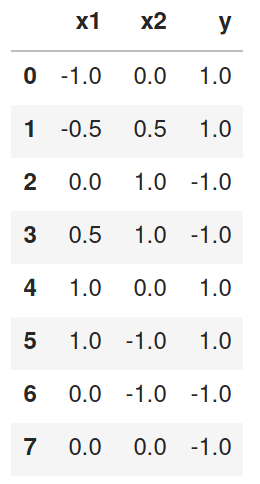
\includegraphics[scale=0.3]{adaboost_points}

\clearpage

I then created the following functions

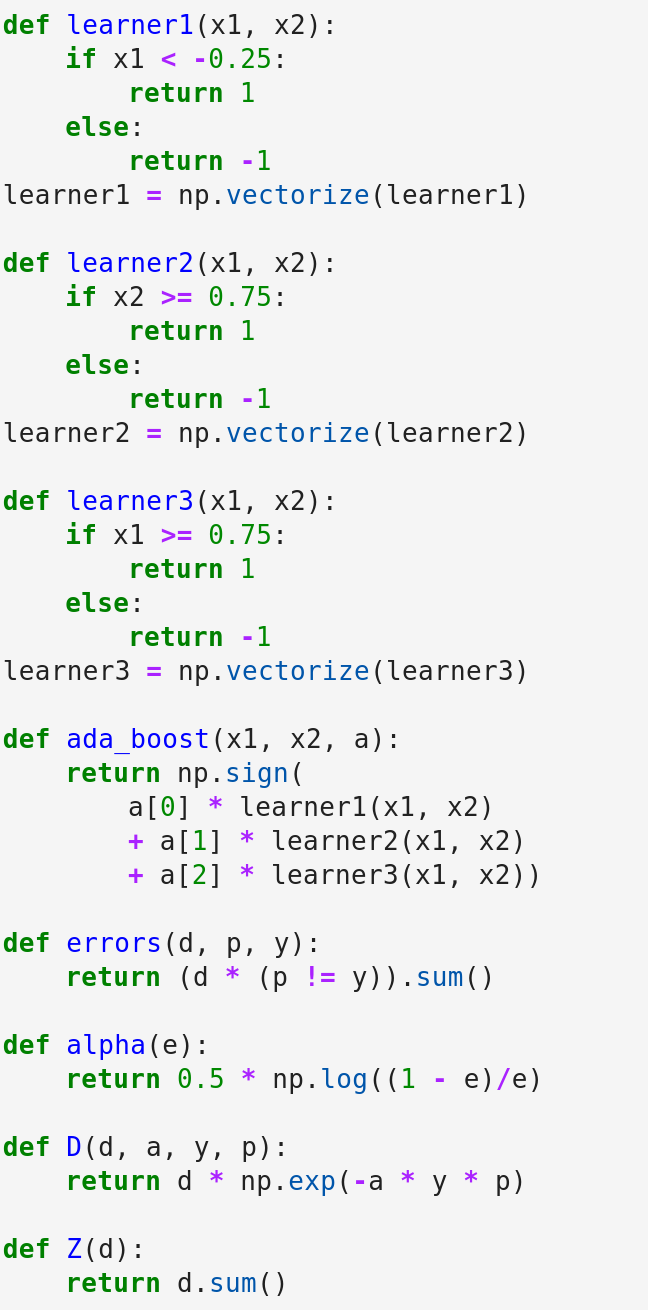
\includegraphics[scale=0.25]{functions}

I used the functions to calculate each iteration, resulting in the following table.

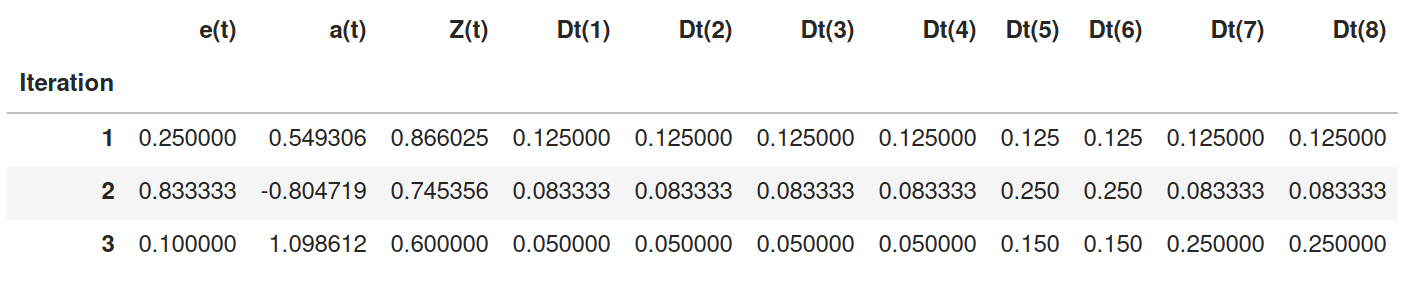
\includegraphics[scale=0.3]{adaboost_iterations}

\clearpage

I then plotted the decision boundary using a meshgrid.

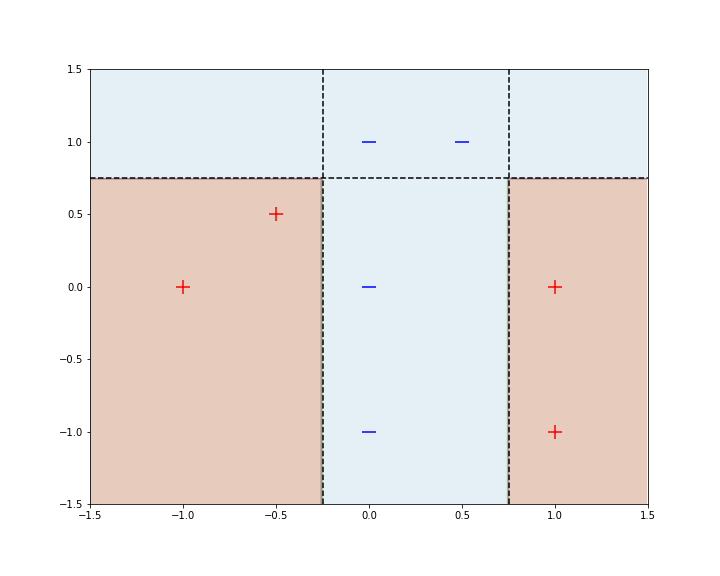
\includegraphics[scale=0.45]{adaboost_boundary}


\item (15 points) What is the training error of this AdaBoost? Give a short explanation for why AdaBoost outperforms a single decision stump.

\end{enumerate}

The training error in this AdaBoost was 0.  The algorithm correctly classified all of the data points.  A decision stump is a decision tree that splits on one value.  AdaBoost outperforms a single decision stump by weighting the arrors of each decistion stump and encorporating those weights into the next iteration when calculating the next decision stump. This allows the algorthim to find the next decision stump by focusing on the points not classified correctly in the prior iteration.


\clearpage 

\item{\bf Linear regression: bias-variance tradeoff, CV, and variable selection} (30 points)


Consider a dataset with $n$ data points $(x^i, y^i)$, $x^i \in \mathbb R^n$, following from the following linear model:
\[
y^i =  {\beta^*}^T x^i + \epsilon^i, \quad i = 1, \ldots, m,
\]
where $\epsilon^i$ are i.i.d. Gaussian noise with \textcolor{red}{zero mean and variance $\sigma^2$}, and $\beta^*$ is the true parameter. Consider the ridge regression as follows:
\begin{equation} \label{1}
\hat \beta(\lambda) 
= \arg\min_{\beta}
\left\{
\frac 1 m \sum_{i=1}^m (y^i - {\beta}^T x^i)^2 + \lambda \|\beta\|_2^2
\right\},
\end{equation}
where $\lambda \geq 0$ is the regularized parameter. 
\begin{enumerate}
\item (5 points) Find the closed form solution for $\hat \beta(\lambda)$ and its distribution conditioning on $\{x^i\}$ (i.e., treat them as fixed).

\vspace{5 mm}

$\frac{\partial{\hat \beta(\lambda)}}{\partial{\beta}} =
\arg\min_{\beta}\left\{-\frac{2}{m}Xy + \frac{2}{m}XX^T\beta + \frac{2\lambda}{m}\beta\right\}$

\vspace{2 mm}
$\frac{\partial{\hat \beta(\lambda)}}{\partial{\beta}} = \arg\min_{\beta}\left\{-2X^T(y - \beta^TX) + 2\lambda\beta\right\} = 0$

\vspace{2 mm}

$\hat\beta(\lambda) = (X^TX + \lambda I)^{-1} X^T y$

\vspace{2 mm}

$\mathbb E[\hat\beta] = (X^TX + \lambda I)^{-1} X^T X \beta^*$, where $\beta^*$ represents the parameters of X, therefore replacing y.

\vspace{2 mm}

$Var[\hat\beta]  = \sigma^2 (X^TX + \lambda I)^{-1} X^T X [(X^TX + \lambda I)^{-1}]^T$

\vspace{2 mm}

Since $\epsilon^i$ is i.i.d. Gaussian, y is also a Gaussian, implying that $\hat \beta$ is also Gaussian, so

$$\hat\beta \sim \mathcal{N}(\mathbb E[\hat\beta],Var[\hat\beta])$$



\item (5 points) Calculate the bias  $\mathbb E[x^T {\hat \beta}(\lambda)] - x^T {\beta^*}$ as a function of $\lambda$ and some fixed test point $x$.

\vspace{5 mm}

bias  $\mathbb E[x^T {\hat \beta}(\lambda)] - x^T {\beta^*} = \mathbb E[x^T {(X^TX + \lambda I)^{-1} X^T y}] - x^T {\beta^*}$

\vspace{2 mm}

Using Probability Theory (thank you simulation notes!)

\vspace{2 mm}

$\mathbb E[\alpha y] = \alpha\mathbb E[y] = \alpha X \beta^*$

\vspace{2 mm}

The above 

\vspace{2 mm}

$\mathbb E[x^T {(X^TX + \lambda I)^{-1} X^T y}] - x^T {\beta^*}$

\vspace{2 mm}

becomes

\vspace{2 mm}

$x^T {(X^TX + \lambda I)^{-1} X^T X {\beta^*}} - x^T {\beta^*}$

\vspace{5 mm}

\item (5 points) Calculate the variance term $\mathbb E\left[\left(x^T {\hat \beta}(\lambda) - \mathbb E[x^T {\hat \beta}(\lambda)] \right)^2\right]$ as a function of $\lambda$.

\vspace{5 mm}

$Var[x^T\hat\beta] = x^T Var[\hat\beta] x$

$Var[\hat\beta]  = \sigma^2 (X^TX + \lambda I)^{-1} X^T X [(X^TX + \lambda I)^{-1}]^T$

$Var[x^T\hat\beta]  = x^T \sigma^2 (X^TX + \lambda I)^{-1} X^T X [(X^TX + \lambda I)^{-1}]^T x$

\item (5 points) Use the results from parts (b) and (c) and the bias-variance decomposition to analyze the impact of $\lambda$ in the \textcolor{red}{mean} squared error. Specifically, which term dominates when $\lambda$ is small, and large, respectively?

$MSE = [bias  \mathbb E[x^T {\hat \beta}(\lambda)] - x^T {\beta^*}]^2 + \mathbb E\left[\left(x^T {\hat \beta}(\lambda) - \mathbb E[x^T {\hat \beta}(\lambda)] \right)^2\right] + \epsilon$

\vspace{2 mm}

$= [x^T {(X^TX + \lambda I)^{-1} X^T X {\beta^*}}(\lambda) - x^T {\beta^*}]^2 + x^T \sigma^2 (X^TX + \lambda I)^{-1} X^T X [(X^TX + \lambda I)^{-1}]^T x$ 
\vspace{5 mm}


When $\lambda$ is large the bias dominates, when $\lambda$ is small, the variance dominates. This is what is known as the bias variance tradeoff.

\vspace{5 mm}

\item (5 points) Now suppose we have $m= 100$ samples. Write a pseudo-code to explain how to use cross validation to find the optimal $\lambda$.

\vspace{5 mm}

Below is a description of the procedure using leave one out cross validation (LOOCV).

\begin{enumerate}
	\item Define a range for the penalty parameter $\lambda$
	\item m = 100, for i in \{1 to M\}, Divide the set into samples \{1, ..., m\} leaving out i and, \{i\} respectively 
	\item Fit the ridge regression model for each $\lambda$ using the training set to obtain $\hat \beta_{-i}(\lambda)$ and $\hat \sigma_{-i}^2(\lambda)$
	\item Evaluate the prediction error of $\left\lvert|Y_{i} - X_{i}, *\hat \beta_{-i}\right\rvert$.
	\item repeat steps 1 through 3 until iteration is complete
	\item average the prediction performances of the test sets to get the cross validated log likelhood
	\item the value of $\lambda$ that maximizes the cross validated log likelihood is the the optimal $\lambda$.
\end{enumerate}

\vspace{5 mm}

\item (5 points) Explain if we would like to perform variable selection, how should we \textcolor{red}{change} the regularization term in Equation (\ref{1}) to achieve this goal. 


\begin{equation} \label{1}
\theta^r
= \arg\min_{\theta} L(\theta)=
\left\{
\frac 1 m \sum_{i=1}^m (y^i - {\theta}^T x^i)^2 + \lambda \|\theta\|_1
\right\}
\end{equation}

\end{enumerate}



\clearpage

\item {\bf Random forest and one-class SVM for email spam classifier} (40 points)

Your task for this question is to build a spam classifier using the UCR email spam dataset \url{https://archive.ics.uci.edu/ml/datasets/Spambase} came from the postmaster and individuals who had filed spam. Please download the data from that website. The collection of non-spam emails came from filed work and personal emails, and hence the word \textsf{'george'} and the area code \textsf{'650'} are indicators of non-spam. These are useful when constructing a personalized spam filter. You are free to choose any package for this homework. Note: there may be some missing values. You can just fill in zero.

\begin{enumerate}

\item (10 points) Build a CART model and visualize the fitted classification tree.

I first tuned my tree depth measuring the Area Under the ROC Curve and decided on a max depth of 6 (5 + 1 since index starts at 0).

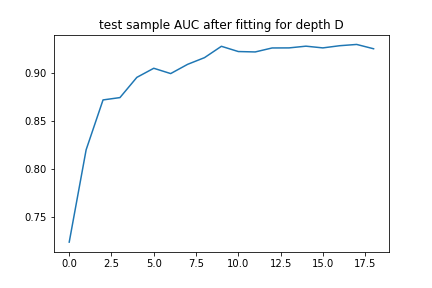
\includegraphics[scale=0.5]{tune_dectree_depth}

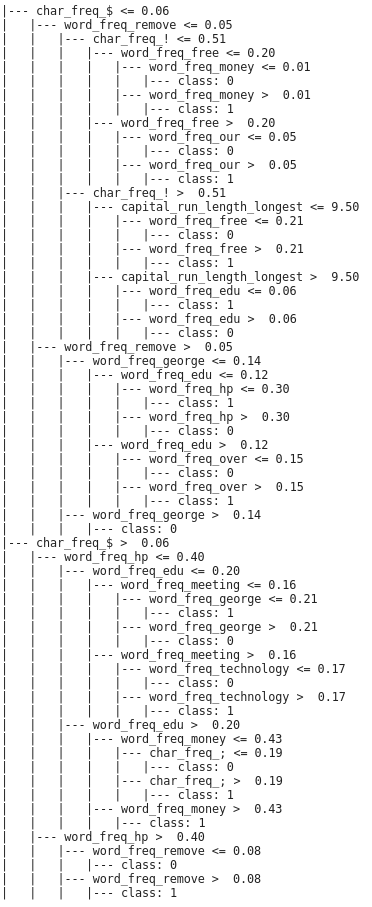
\includegraphics[scale=0.5]{spam_text_tree}

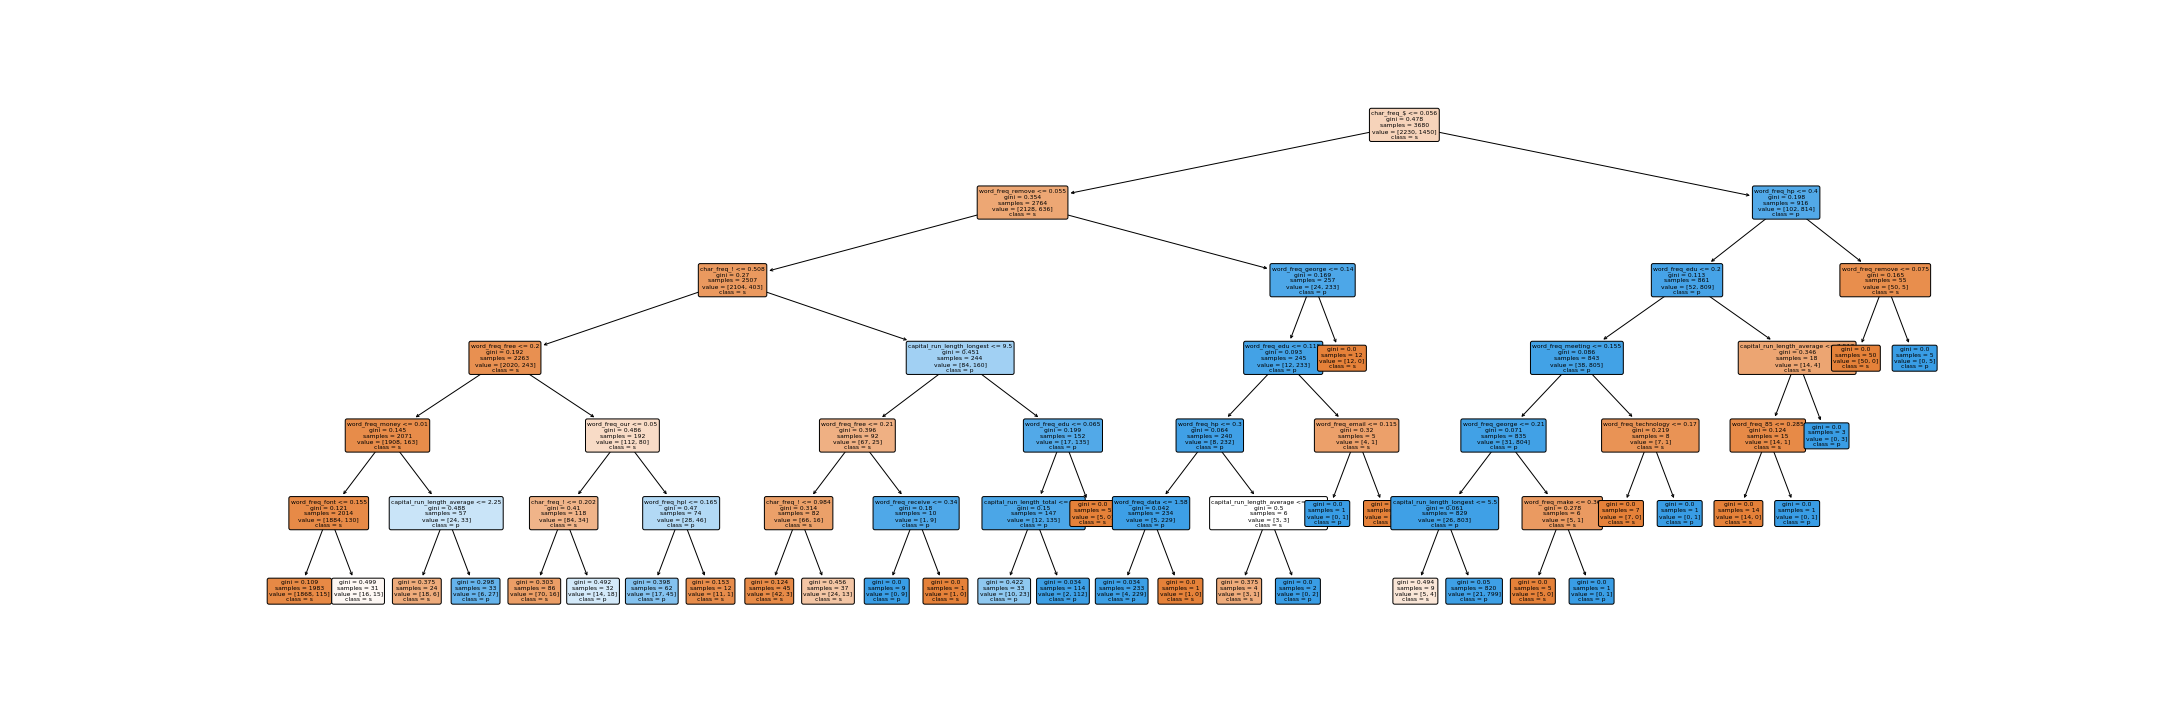
\includegraphics[scale=0.2]{spam_tree}

\clearpage

\item (15 points) Now also build a random forest model. Partition the data to use the first 80\% for training and the remaining 20\% for testing. Compare and report the test error for your classification tree and random forest models on testing data. Plot the curve of test error (total misclassification error rate) versus the number of trees for the random forest, and plot the test error for the CART model (which should be a constant with respect to the number of trees). 

\vspace{5 mm}

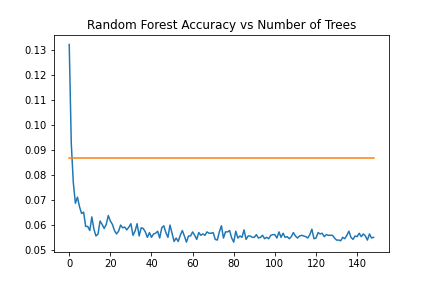
\includegraphics[scale=0.6]{spam_rf150}

The error rate for The Decision Tree algorithm is 0.0858.  Iterating through random forests of trees between 1 and 150, the error rate drops from 0.0986 with one decision tree, and starts to converge at 12 trees with an error rate of 0.0549.

\vspace{5 mm}

\item (15 points) Now we will use a one-class SVM approach for spam filtering. Partition the data to use the first 80\% for training and the remaining 20\% for testing. Extract all {\it non-spam} emails from the training block (80\% of data you have selected) to build the one-class kernel SVM using RBF kernel (you can turn the kernel bandwidth to achieve good performance). Then apply it on the 20\% of data reserved for testing (thus this is a novelty detection situation), and report the total misclassification error rate on these testing data. 

\vspace{5 mm}

I normalized the testing set using sklearn's standard scaler.  I randomly split the data into 80\% train and 20\% test.  I calculated my gamma using the median trick on the 80\% training data (including spam and not spam).  I then also calculation my spam ratio (spam / total count) in order to tune the nu parameter. I fit only the not spam data from my 80\% training sample into the One-Class SVM Classifier, then predicted the remaining 20\% testing set.  The total misclassification rate was 0.4234.  The default gamma='scale' parameter in sklearn's one class SVM classifier performed better than using the median trick, and had a total misclassification rate of 0.4083.

\end{enumerate}


\end{enumerate}





\end{document}
